\chapter{Outils de programmation pour la robotique}\label{ch:hatchery}
\setlength{\epigraphwidth}{0.78\textwidth}
\epigraph{``L'espoir est que, dans quelques années, les cerveaux humains et les machines informatiques seront très étroitement couplés et que le partenariat qui en résultera pensera comme aucun cerveau humain n'a jamais pensé et traitera les données d'une manière qui n'est pas abordée par les machines de traitement de l'information que nous connaissons aujourd'hui.''}{\begin{flushright}--Joseph \citet{licklider1960man}, \href{https://groups.csail.mit.edu/medg/people/psz/Licklider.html}{\textit{Symbiose homme-ordinateur}}\end{flushright}}

Dans ce chapitre, nous aborderons la conception et la mise en œuvre d'un environnement de développement intégré (EDI) pour la construction de logiciels robotiques intelligents. Les robots modernes sont de plus en plus pilotés par des systèmes qui apprennent et s'améliorent au fil du temps. La plupart des chercheurs s'accordent à dire que les systèmes robotiques modernes n'ont pas encore atteint des capacités sensorimotrices biologiquement compétitives et que la plupart des systèmes intelligents ne sont pas physiquement incorporés. Cependant, nous estimons que tout système de contrôle en boucle fermée qui n'est pas explicitement programmé pour effectuer une tâche spécifique, mais qui l'apprend par expérience est un \textit{système intelligent}. De plus, tout système en boucle fermée avec des moteurs physiques est un \textit{système robotique}. Bien que la recherche ait démontré des applications réussies dans ces deux domaines séparément, il est largement admis que l'intégration des systèmes intelligents et de la robotique sera extrêmement fructueuse lorsqu'elle sera pleinement réalisée.

Hatchery est un outil conçu pour aider les programmeurs à écrire des applications robotiques en utilisant le middleware ROS. Au moment de sa sortie, \href{https://github.com/duckietown/hatchery}{Hatchery} était le premier plugin ROS pour la \href{https://www.jetbrains.org/intellij/sdk/docs}{IntelliJ Platform} \footnote{Une plateforme EDI pour le développement C/C++, Python et Android, entre autres.}, et aujourd'hui, est la plus utilisée avec plus de 10 000 téléchargements uniques. Bien que l'idée soit simple, son absence antérieure et son adoption ultérieure suggèrent qu'il existe une demande non satisfaite pour de tels outils dans le développement de systèmes logiciels intelligents, en particulier dans les applications spécifiques à un domaine comme la robotique.
%

\begin{figure}
    \centering
    \begin{tikzpicture}
        \begin{axis}[
            ybar, ymin=0,
            ylabel=Downloads,
            date coordinates in=x,
            xmin=2017-12-01,
            xmax=2019-06-01,
            xtick=data,
            xticklabel style={
                rotate=70,
                anchor=near xticklabel,
            },
            xticklabel=\year-\month,
            nodes near coords,
            nodes near coords align={vertical},
            height=0.25\textwidth,
            width=0.95\textwidth,
            enlarge x limits=0.03,
            axis x line*=bottom,
            axis y line*=left,
            tick pos=left,
            compat=newest,
        ]
            \addplot table[col sep=comma, x=Category,y=Downloads]{../data/hatchery_downloads.csv};
        \end{axis}
        \node[above,font=\large\bfseries] at (current bounding box.north) {Unique downloads of Hatchery};
    \end{tikzpicture}
    \caption{Unique downloads of Hatchery between the time of its release and June 2019. \url{https://plugins.jetbrains.com/plugin/10290-hatchery}.}
    \label{fig:hatchery_downloads}
\end{figure}
%
\section{Introduction à ROS}

Le système d'exploitation \href{https://www.ros.org/}{Robot Operating System} (ROS)~\citep{quigley2009ros} est un intergiciel populaire pour les applications robotiques. Il fournit une infrastructure logicielle pour la messagerie distribuée, mais comprend également un ensemble de bibliothèques et d'outils graphiques développés par la communauté pour la création d'applications robotiques. ROS n'est pas un système d'exploitation (OS) au sens traditionnel du terme, mais il prend en charge des fonctionnalités similaires telles que la mémoire partagée et la communication entre processus. Contrairement aux systèmes purement axés sur les messages tels que DDS~\citep{pardo2003omg} et \href{https://zeromq.org/}{ZMQ}~\citep{hintjens2013zeromq}, ROS fournit, outre l'infrastructure de communication, des API spécifiques pour la construction de systèmes robotiques décentralisés, notamment ceux qui sont capables de se déplacer. Cela comprend des bibliothèques standard pour la sérialisation et la désérialisation de données géométriques, de cadres de coordonnées, de cartes, de messages de capteurs et d'images.

Le middleware ROS fournit plusieurs frontaux de langage pour la programmation polyglotte. Selon un recensement communautaire effectué en 2018, 55\% de toutes les applications ROS sur GitHub sont écrites en C/C++, suivies par Python avec une part de 25\% de développeurs. Le code source d'une application ROS typique contient un mélange de code C/C++ et Python, correspondant aux préférences linguistiques respectives des communautés de la robotique et de l'apprentissage machine. Hatchery est compatible avec la plupart des bibliothèques clientes ROS courantes, notamment \href{https://wiki.ros.org/rosjava}{rosjava} pour Java, \href{https://wiki.ros.org/rospy}{rospy} pour Python, \href{https://wiki.ros.org/rospy}{roscpp} pour C/C++, et d'autres frontaux de langage.

\begin{figure}
    \centering
    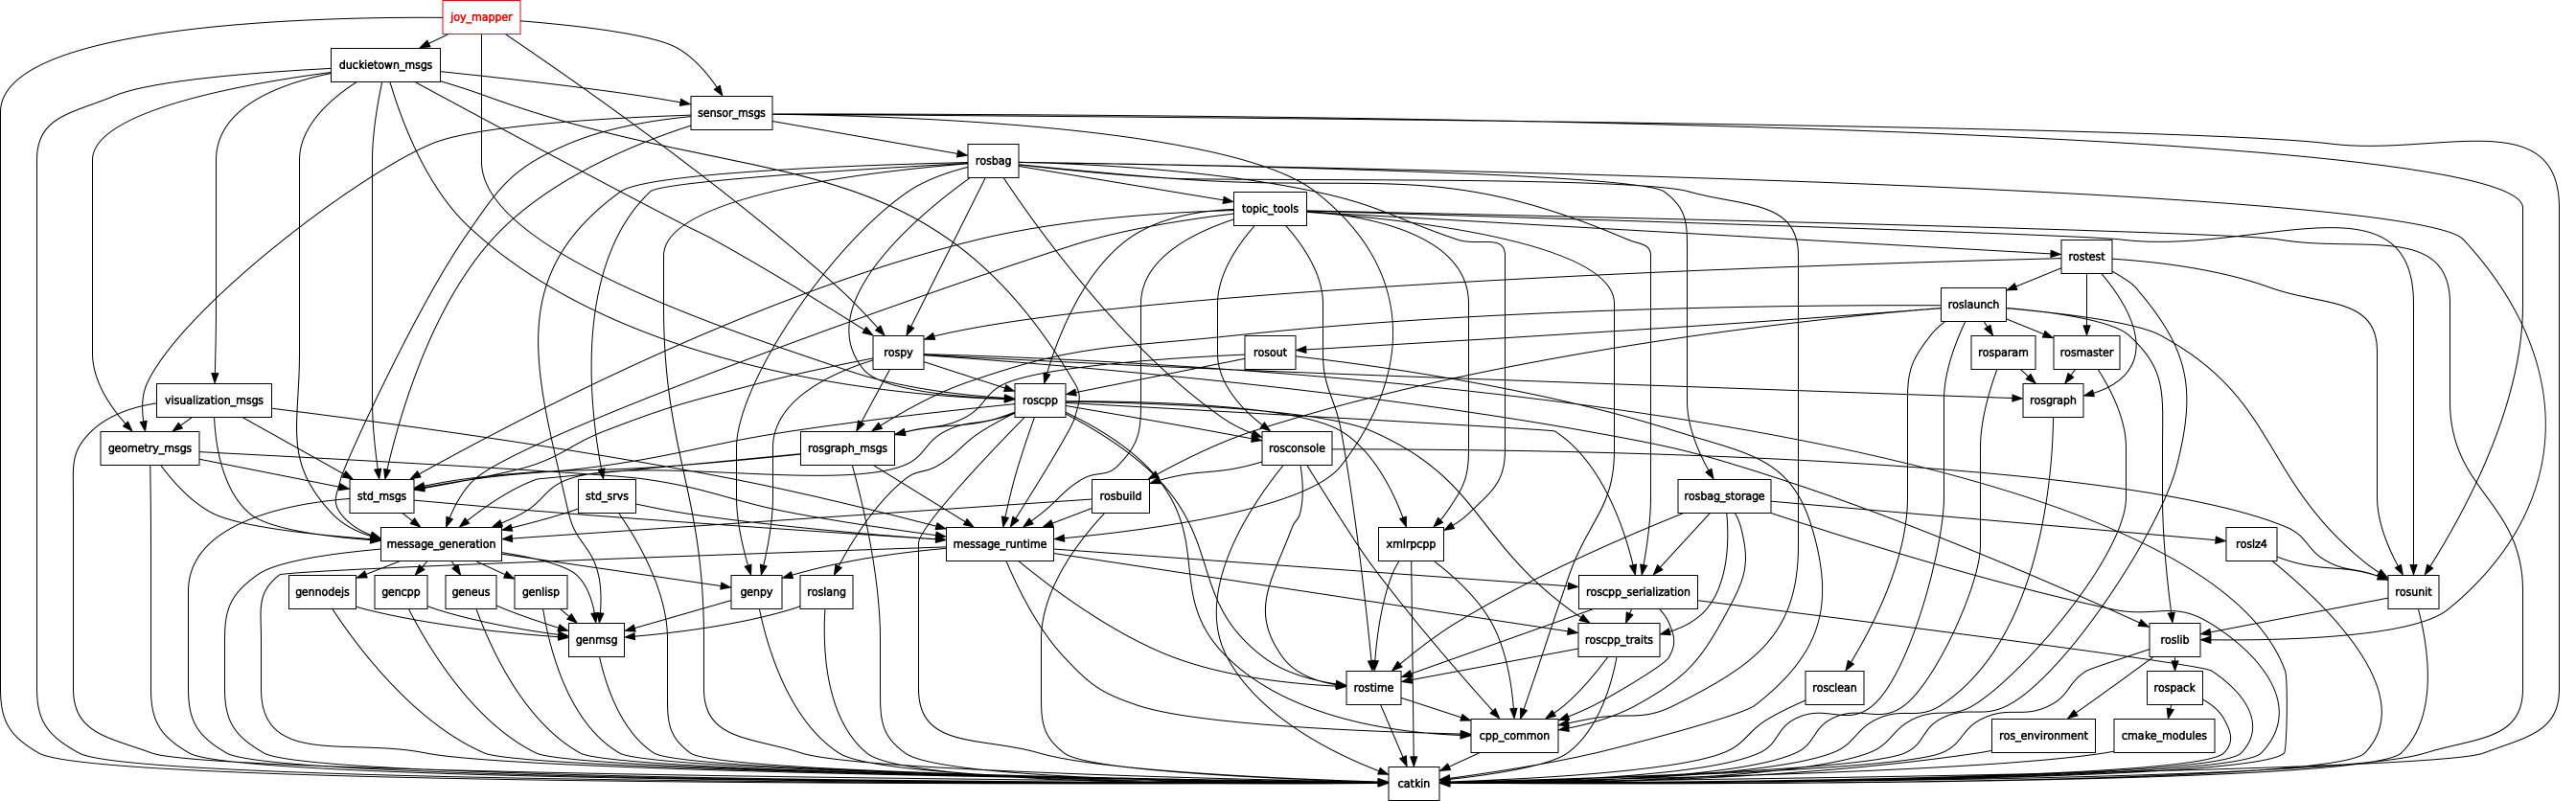
\includegraphics[width=\textwidth]{../figures/rqt_dep_graph.png}
    \caption{Une application ROS typique contient un grand graphique de dépendances.}
\end{figure}

Un projet ROS typique comporte plusieurs composantes, dont le code source, les fichiers de configuration, l'infrastructure de construction, les artefacts compilés et l'environnement de déploiement. Pour construire une application ROS simple, plusieurs étapes sont nécessaires. Tout d'abord, il faut installer le système ROS, qui n'est officiellement supporté que sur les distributions Linux basées sur Debian.\hspace{-.08em}\footnote{Les instructions détaillées d'installation peuvent être trouvées ici : \url{https://wiki.ros.org/ROS/Installation}}
%
En supposant que le ROS a été installé à l'emplacement par défaut, il peut être localisé comme tel :
%
\begin{pclisting}
    ~$ source /opt/ros/<ROS DISTRO>/setup.[ba]sh
\end{pclisting}
%
Une application ROS minimale contient au moins un \textit{éditeur} et un \textit{abonné}, qui font passer les messages sur un canal de communication partagé. L'éditeur peut être défini comme suit :
%
\begin{pythonlisting}[title=./catkin\_ws/src/pubsub/publisher.py]
import rospy
from std_msgs.msg import String

pub = rospy.Publisher("(*@\hl{channel}@*)", String, queue_size=10)
rospy.init_node("publisher", anonymous=True)
rate = rospy.Rate(10)
while not rospy.is_shutdown():
pub.publish("Some message")
rate.sleep()
\end{pythonlisting}
%
Au fur et à mesure que l'éditeur écrit des messages sur \hl{\ttfamily{\canal de petite taille}, un autre noeud qui est abonné au même canal recevra un rappel lorsque de nouveaux messages arriveront et pourra les lire sur le canal :
%
\begin{pythonlisting}[title=./catkin\_ws/src/pubsub/subscriber.py]
def callback(data):
    rospy.loginfo(rospy.get_caller_id() + "received data %s", data.data)

    rospy.init_node("subscriber", anonymous=True)
    rospy.Subscriber("(*@\hl{channel}@*)", String, callback)
    rospy.spin()
\end{pythonlisting}
%
Tous les paquets ROS ont un fichier de lancement, qui contient un manifeste des nœuds disponibles :
%
\begin{launchlisting}[title=./catkin\_ws/src/pubsub/pubsub.launch]
<launch>
<node name="publisher" pkg="pubsub" type="publisher.py" output="screen"/>
<node name="subscriber" pkg="pubsub" type="subscriber.py" output="screen"/>
</launch>
\end{launchlisting}
%
Pour construire et exécuter l'application, les séries de commandes suivantes sont nécessaires :
%
\begin{pclisting}
    ~$ cd catkin_ws && catkin_make
\end{pclisting}
%
\begin{pclisting}
~$ roslaunch pubsub pubsub.launch
\end{pclisting}
%
Plutôt que d'interagir avec la ligne de commande, il serait pratique de disposer d'un outil graphique permettant d'effectuer toutes ces tâches automatiquement. En outre, il serait utile de détecter s'il y a une erreur typographique ou une référence de navigation dans le fichier de lancement :
%
\begin{launchlisting}[title=./catkin\_ws/src/pubsub/pubsub.launch]
<launch>
<node name="publisher" pkg="pubsub" type="(*@\color{red}\textbf{pubsher.py}@*)" output="screen"/>
<node name="subscriber" pkg="pubsub" type="(*@\color{blue}\underline{subscriber.py}@*)" output="screen"/>
</launch>
\end{launchlisting}
%
Remarquez que l'erreur typographique est imprimée en rouge et que la référence de fichier valide est soulignée en bleu, indiquant qu'elle peut être sélectionnée pour ouvrir le fichier indiqué ci-dessus. En gros, ce sont les types de fonctionnalités que les EDI fournissent et sont des exemples de fonctionnalités spécifiques à Hatchery.

\section{Installation}\label{subsec:installation}

\noindent Pour utiliser simplement l'outil, les utilisateurs doivent avoir les dépendances logicielles suivantes :
%
\begin{enumerate}
\item MacOS ou une distribution Linux basée sur Debian
\item Robot Operating System (Electric Emys or later)
\item Java SE (JRE 8+) ou CLion/PyCharm 2019.1+
\end{enumerate}
%
\noindent Les utilisateurs de ROS peuvent utiliser la commande suivante pour ouvrir un projet ROS existant :
%
\begin{pclisting}
~$ git clone https://github.com/duckietown/hatchery && cd hatchery &&
./gradlew runIde [-Project="<ABSOLUTE_PATH_TO_ROS_PROJECT>"]].
\end{pclisting}
%
\noindent Les utilisateurs de Duckietown peuvent simplement utiliser la coquille de Duckietown :
%
\begin{dtslisting}
dt> hatchery
\end{dtslisting}
%
\noindent Hatchery peut également être installé directement depuis l'intérieur des EDI CLion ou PyCharm, via les options de menu suivantes : \menu{File > Settings > Plugins > Marketplace > {\faSearch ``Hatchery''}}

\section{Développement de plugins}

Pour construire un EDI, certains outils sont utiles. Tout d'abord, il y a un EDI et son code source. Supposons que l'EDI\textsubscript{0} existe. Afin de construire un nouvel EDI, EDI\textsubscript{1}, nous pouvons charger le code source de l'EDI\textsubscript{0} dans l'EDI\textsubscript{0} et utiliser l'EDI\textsubscript{0}, pour modifier, compiler et ré-exécuter le code, qui devient l'EDI\textsubscript{1}, dans lequel le processus est répété. Cette approche présente toutefois quelques inconvénients. Tout d'abord, la plupart des EDI sont déjà assez lourds à compiler et à exécuter. Comme la plupart des fonctionnalités auxiliaires sont petites en comparaison, les EDI modernes ont adopté une conception modulaire, qui leur permet de charger des paquets spécifiques (c'est-à-dire des \ \textit{plugins}) selon les besoins. Ainsi, la plupart des développeurs peuvent sauter la première étape et charger leur plugin directement dans l'EDI \textsubscript{0}. Il est toujours pratique d'avoir le code source de la plate-forme à titre de référence, mais dans la plupart des cas, ce code est en lecture seule.

Hatchery utilise la \href{https://www.jetbrains.org/intellij/sdk/docs/}{IntelliJ Platform}, une plateforme EDI qui supporte la plupart des langages de programmation courants. En ciblant une plateforme EDI qui prend en charge la programmation polyglotte, Hatchery est en mesure de se concentrer sur les caractéristiques agnostiques des langages dans l'écosystème ROS, telles que l'analyse et l'édition de fichiers de configuration spécifiques aux ROS, la configuration de la construction et de l'exécution et d'autres tâches de développement courantes.

\subsection{Refactoring}\label{subsec:refactoring}

Le remaniement est une caractéristique essentielle de tout EDI, et l'essence du remaniement est le changement de nom. Considérez ce qui doit se produire lorsqu'un utilisateur souhaite renommer un jeton dans son programme, comme le paramètre nommé \inline{data} sur la ligne \#1 ci-dessous :
%
\begin{pythonlisting}
def callback(data):
    rospy.loginfo(rospy.get_caller_id() + "received data: %s", data.data)
\end{pythonlisting}
%
Si elle utilisait l'éditeur de texte \inline{vim}, une solution serait de remplacer toutes les occurrences textuelles de la chaîne \inline{data} dans le fichier en utilisant \inline{:\%s/data/msg/g}, ce qui donnerait le résultat suivant :

\begin{pythonlisting}
def callback((*@\hl{msg}@*)):
    rospy.loginfo(rospy.get_caller_id() + "received (*@\hl{msg}@*): %s", (*@\hl{msg}@*).(*@\hl{msg}@*))
\end{pythonlisting}
%
Il y a eu quatre occurrences de la chaîne \inline{data}, dont seulement deux ont été correctement renommées. Au lieu de cela, seules les chaînes qui font référence au paramètre de fonction doivent être renommées :

\newcommand{\cfbox}[2]{\colorlet{\currentcolor}{.}{\color{#1}\fbox{\color{\currentcolor}#2}}}

\begin{pythonlisting}
def callback((*@\cfbox{red}{data}@*)):
    rospy.loginfo(rospy.get_caller_id() + "received data: %s", (*@\cfbox{red}{data}@*).data)
\end{pythonlisting}
%
En général, nous aimerions pouvoir renommer les identificateurs d'un fichier à l'autre et d'une langue à l'autre. Pour ce faire, nous avons besoin d'une compréhension plus riche du code qui transcende le texte -- nous avons besoin d'un analyseur.

\subsection{Analyse syntaxique}\label{subsec:the-parser}

L'un des composants les plus importants et les moins appréciés d'un EDI est l'analyseur syntaxique. Contrairement aux compilateurs, la plupart des EDI n'utilisent pas l'analyse récursive par descente ou par réduction de décalage comme le traitent la plupart des manuels de compilation~\citep{appel2003modern}, car ces algorithmes ne sont pas bien adaptés à l'édition en temps réel du code source. Les modifications sont généralement courtes et localisées à l'intérieur d'un gros fichier, et sont souvent invalides ou incomplètes entre les frappes. Comme la plupart des EDI sont censés se remettre des erreurs locales et fournir un retour d'information réactif pendant l'édition du code source, il serait coûteux et inutile de préparer à nouveau l'ensemble du programme entre deux éditions mineures. Afin d'analyser le code source en cours de modification simultanée et de fournir un retour d'information interactif, il faut veiller tout particulièrement à assurer une analyse robuste et réactive.

Diverses techniques ont été développées pour améliorer la réactivité des analyseurs modernes. Les techniques d'analyse incrémentielle comme celles proposées pour la première fois dans \citet{ghezzi1979incremental} et développées plus avant par \citet{wagner1997practical,wagner1997incremental} cherchent à intégrer la mise en cache et l'analyse différentielle pour accélérer l'analyse des programmes soumis à des modifications simultanées. Les techniques d'analyse floue comme celles décrites dans ~\citet{koppler1997systematic} visent à accroître la flexibilité et la robustesse de l'analyse en présence d'erreurs locales. Ces deux techniques ont joué un rôle dans le développement d'outils de programmation sensibles au langage, qui doivent être capables de fournir un retour d'information rapide et spécifique pendant que l'utilisateur tape.

Les instructions de procédure des analyseurs modernes sont rarement écrites à la main, sauf si le langage analysé est très simple ou si l'on souhaite obtenir des performances brutes. Même les analyseurs conçus pour les EDI, où l'analyse incrémentale et la tolérance aux erreurs sont si importantes, les boîtes à outils de métacompilation telles que ANTLR~\citep{parr1995antlr}, ou Xtext~\citep{eysholdt2010xtext} couvrent un nombre surprenant de cas d'utilisation courants. Hatchery utilise \href{https://github.com/JetBrains/grammar-kit}{Grammar-Kit}, une boîte à outils conçue pour aider les utilisateurs à développer des plugins linguistiques personnalisés pour la \href{https://www.jetbrains.org/intellij/sdk/docs}{Plateforme IntelliJ}. Il utilise un générateur de lexique basé sur DFA, JFlex~\citep{klein2001jflex}, et un générateur d'analyseur personnalisé basé sur la grammaire d'expression d'analyse (PEG)~\citep{ford2004parsing}, un descendant de la spécification grammaticale Backus-Naur Form (BNF). Cette spécification est consommée par le générateur d'analyseur GrammarKit et traduite en code source Java, produisant un analyseur qui lit le code source écrit dans le langage spécifié et construit une interface de structure de programme (PSI), la structure de données interne de la plate-forme IntelliJ pour représenter les arbres syntaxiques abstraits (AST). Voici un extrait d'une grammaire PEG BNF pour l'analyse des fichiers ROS \href{https://wiki.ros.org/msg}{\inline{.msg}} :
%
\begin{bnflisting}
rosInterfaceFile ::= ( property | COMMENT )*
property ::= ( TYPE FIELD SEPARATOR CONSTANT ) | ( TYPE FIELD ) {
    pin=3 // Identifie un délimiteur non ambigu ou un point de repli
    recoverWhile="recover_property" // Prédicat de récupération d'erreur
    mixin="edu.umontreal.hatchery.psi.impl.RosMsgNamedElementImpl"
    implements="edu.umontreal.hatchery.psi.RosMsgNamedElement"
    methods=[getType getKey getValue getName setName getNameIdentifier]
}
private recover_property ::= ! ( TYPE | FIELD | SEPARATOR | COMMENT )
\end{bnflisting}
%
\begin{figure}
\centering
% To regenerate: https://homepage.ruhr-uni-bochum.de/jan.holthuis/posts/using-the-latex-rail-package#manual-compilation-and-latexmk-support
\begin{rail}
( [2] TYPE FIELD ( () | SEPARATOR CONSTANT) ) | ( [1] COMMENT )
\end{rail}
\caption{Schéma de chemin de fer pour la grammaire ci-dessus (se lit de gauche à droite).}
\label{fig:railroad}
\end{figure}
%
Les règles lexicales pour les jetons, \inline{TYPE}, \inline{FIELD}, \inline{CONSTANT} et autres sont définies dans un fichier \inline{.flex} séparé, la \href{https://www.jflex.de/manual.html#Grammar}{Grammaire JFlex}. Vous trouverez ci-dessous un extrait du lexique \inline{.flex} qui l'accompagne :
%
\begin{flexlisting}
TYPE_CHARACTER=[^:=#\ \r\n\t\f\\]
FIELD_CHARACTER=[^:=#\ \r\n\t\f\\]
SEPARATOR_CHARACTER=[:=]
CONSTANT_CHARACTER=[^\r\n\f#]
COMMENT_CHARACTER=#[^\r\n\f]*
\end{flexlisting}

Grammar-Kit consomme ces fichiers et génère le code source Java pour l'analyse des fichiers ROS \href{https://wiki.ros.org/msg}{\inline{.msg}}. Les sources générées peuvent être affinées manuellement afin de prendre en charge des fonctionnalités plus avancées telles que la récupération d'erreurs plus souple. Pour les langues courantes comme les langages de description d'interface (IDL) que l'on trouve dans les fichiers ROS \href{https://wiki.ros.org/msg}{\inline{.msg}} et \href{https://wiki.ros.org/srv}{\inline{.srv}}, l'analyseur et le lexer générés par défaut sont généralement suffisants. Hatchery est également capable d'analyser les fichiers \href{https://wiki.ros.org/urdf}{URDF}, \href{https://wiki.ros.org/Manifest}{package manifest} et \href{https://wiki.ros.org/roslaunch/XML}{roslaunch} XML.

\subsection{Exécution et débogage}

Le processus de compilation et d'exécution des applications ROS nécessite souvent plusieurs étapes, ex:
%
\begin{pclisting}
~$ . /opt/ros/<DISTRO>/setup.[ba]sh &&
   cd <PROJECT>/catkin_ws &&
   catkin_make &&
   . devel/setup.sh &&
   [export ROS_MASTER_URI=<URI> &&]
   roslaunch [OPTIONS] src/.../<LAUNCH FILE> [ARGUMENTS]"
\end{pclisting}
%
Hatchery fournit une assistance pour la configuration, la construction et l'exécution d'applications ROS dans une interface utilisateur graphique (GUI) personnalisée. Cette interface graphique sert en fait d'enveloppe à l'interface en ligne de commande (CLI) du ROS. Les éléments visuels comme les options de configuration et les drapeaux de ligne de commande sont écrits dans un modèle interne appelé "Run Configuration" (\autoref{fig:ros_run_config}). Lorsqu'une configuration d'exécution est déclenchée manuellement, le modèle interne de Hatchery est sérialisé en une \inline{String}, représentant la commande à exécuter. Cette \inline{String} est ensuite envoyée à un émulateur de terminal, qui invoque la commande et affiche la sortie correspondante.

\begin{figure}
\centering
\frame{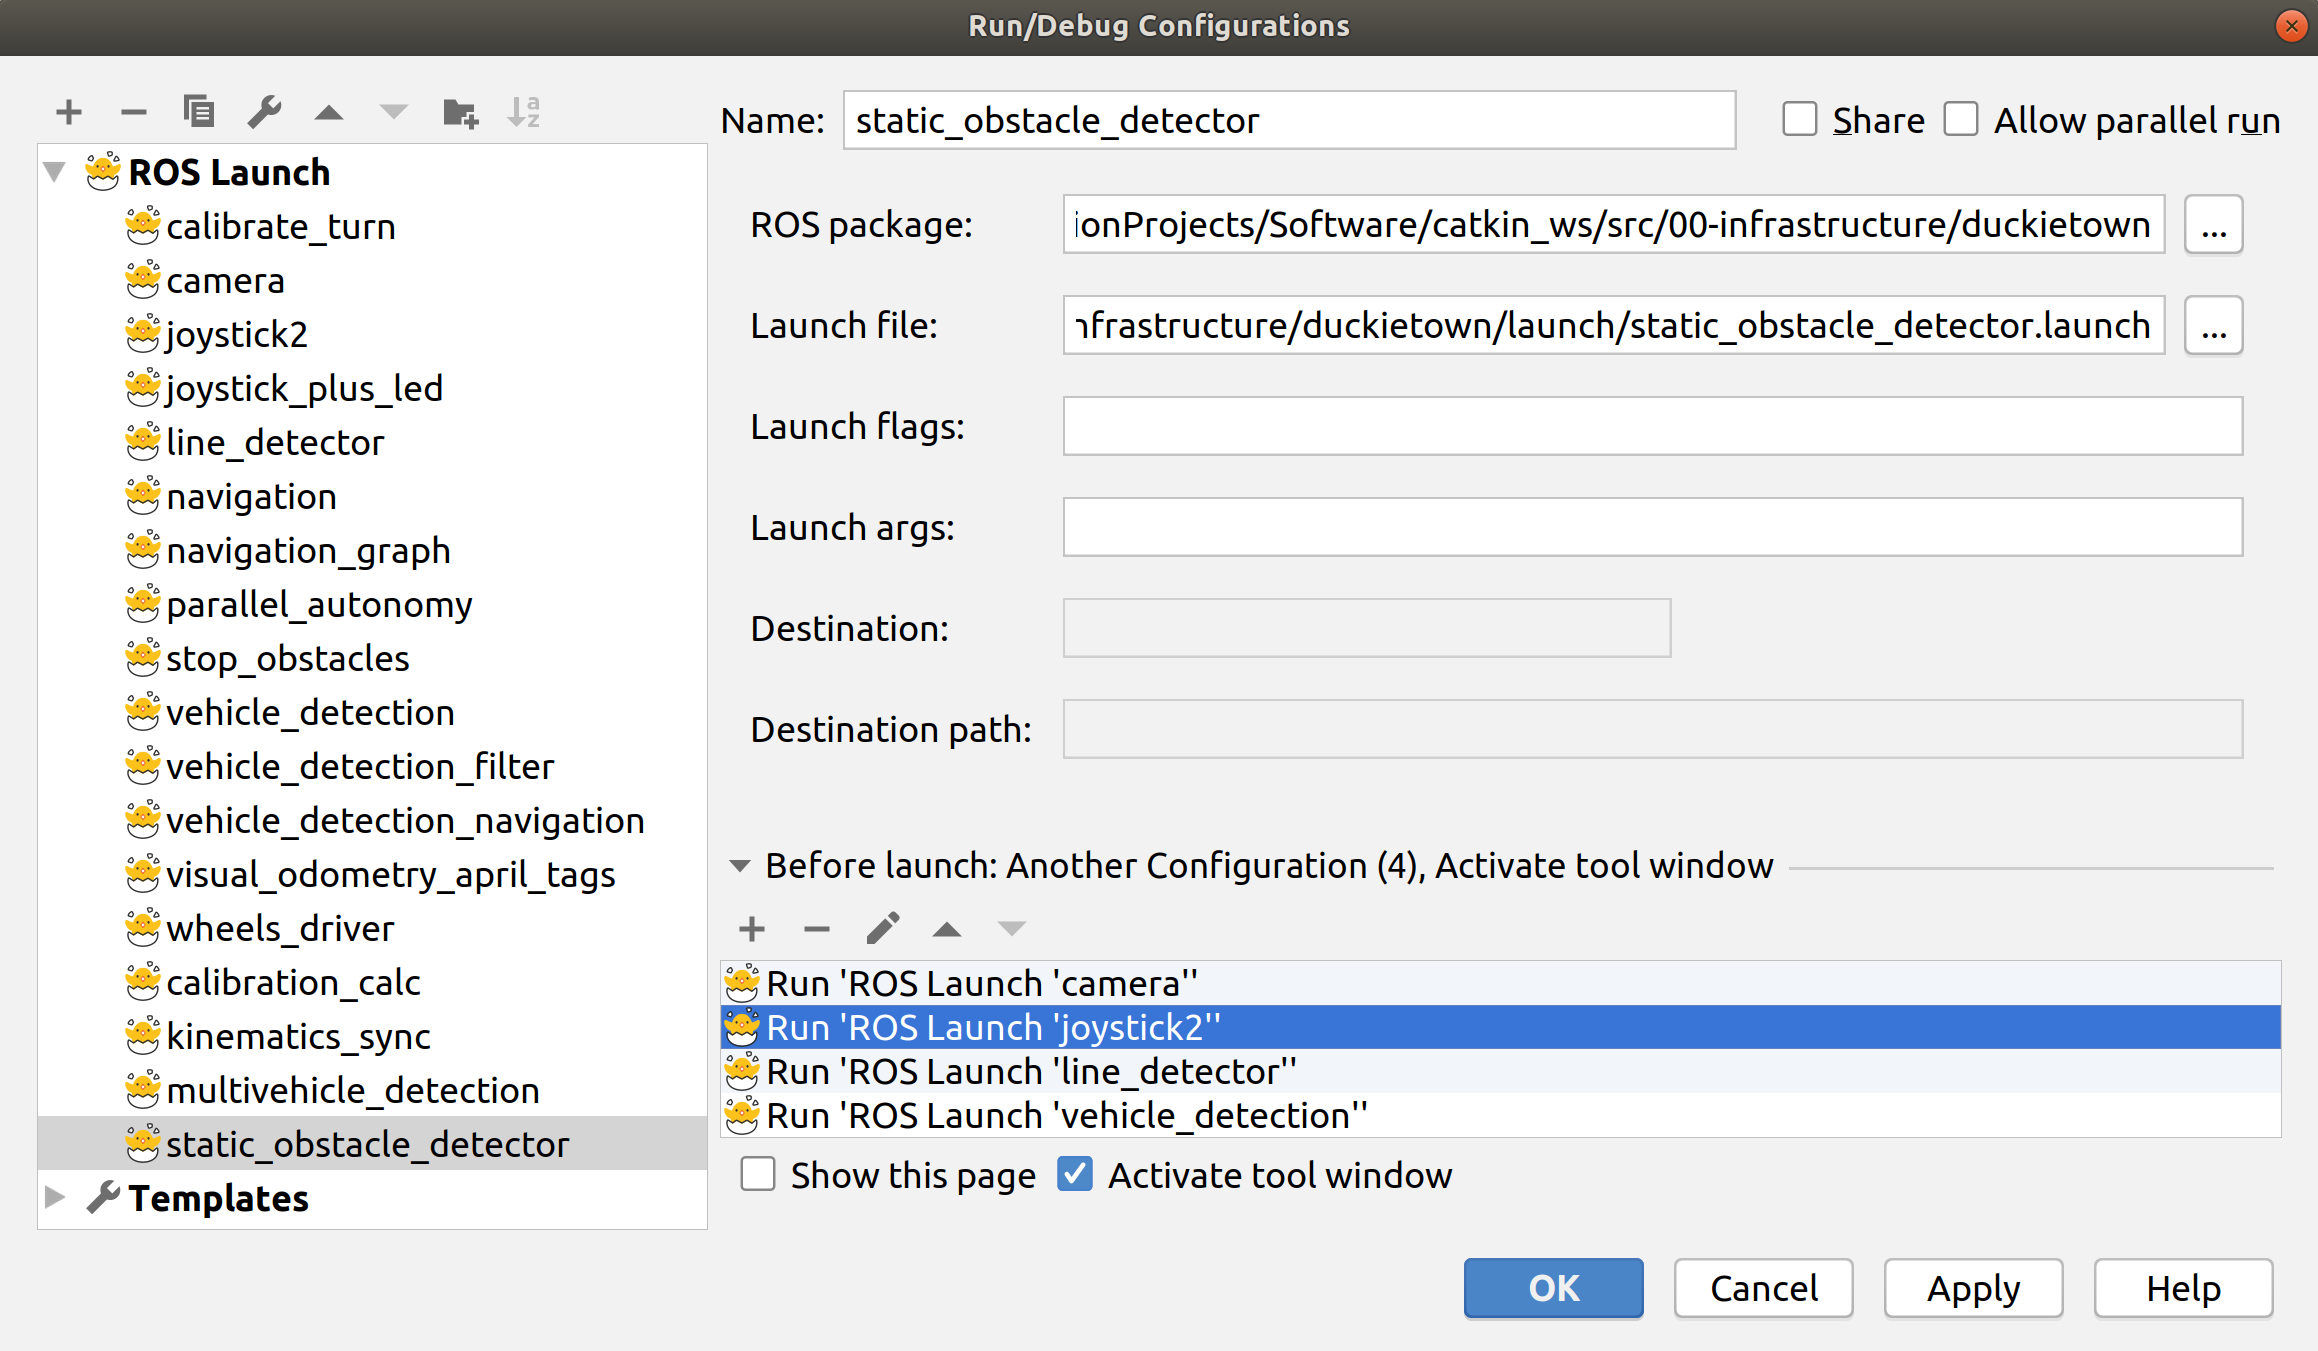
\includegraphics[width=0.90\textwidth]{../figures/ros_run_config.png}}
\caption{ROS Run Configuration. Accessible via: \menu{Run > Edit Configurations > + > ROS Launch}}
\label{fig:ros_run_config}
\end{figure}

\subsection{Interface utilisateur}

Un aspect souvent négligé mais important des outils de développement est l'interface utilisateur graphique, en tant qu'interface principale pour l'édition du code source. Dans les premiers temps de l'informatique moderne, la seule façon de faire entrer ou sortir des informations d'un ordinateur consistait à percer des trous dans le papier~\autoref{fig:evolution_of_programming}. Plus tard, les ordinateurs ont été équipés d'une technologie permettant d'émettre le même motif binaire que les pixels, qui pouvait être utilisé pour afficher un petit alphabet appelé ASCII. Avec des affichages de plus grande densité et fréquence, les ordinateurs pouvaient rendre des formes et des animations plus sophistiquées. Ces améliorations sont le résultat direct de l'innovation graphique, mais peuvent également être considérées comme des progrès dans la représentation des programmes, où le support symbolique n'était lui-même qu'une convention notationnelle que les développeurs et les machines utilisaient pour communiquer.

\begin{figure}
\center
% 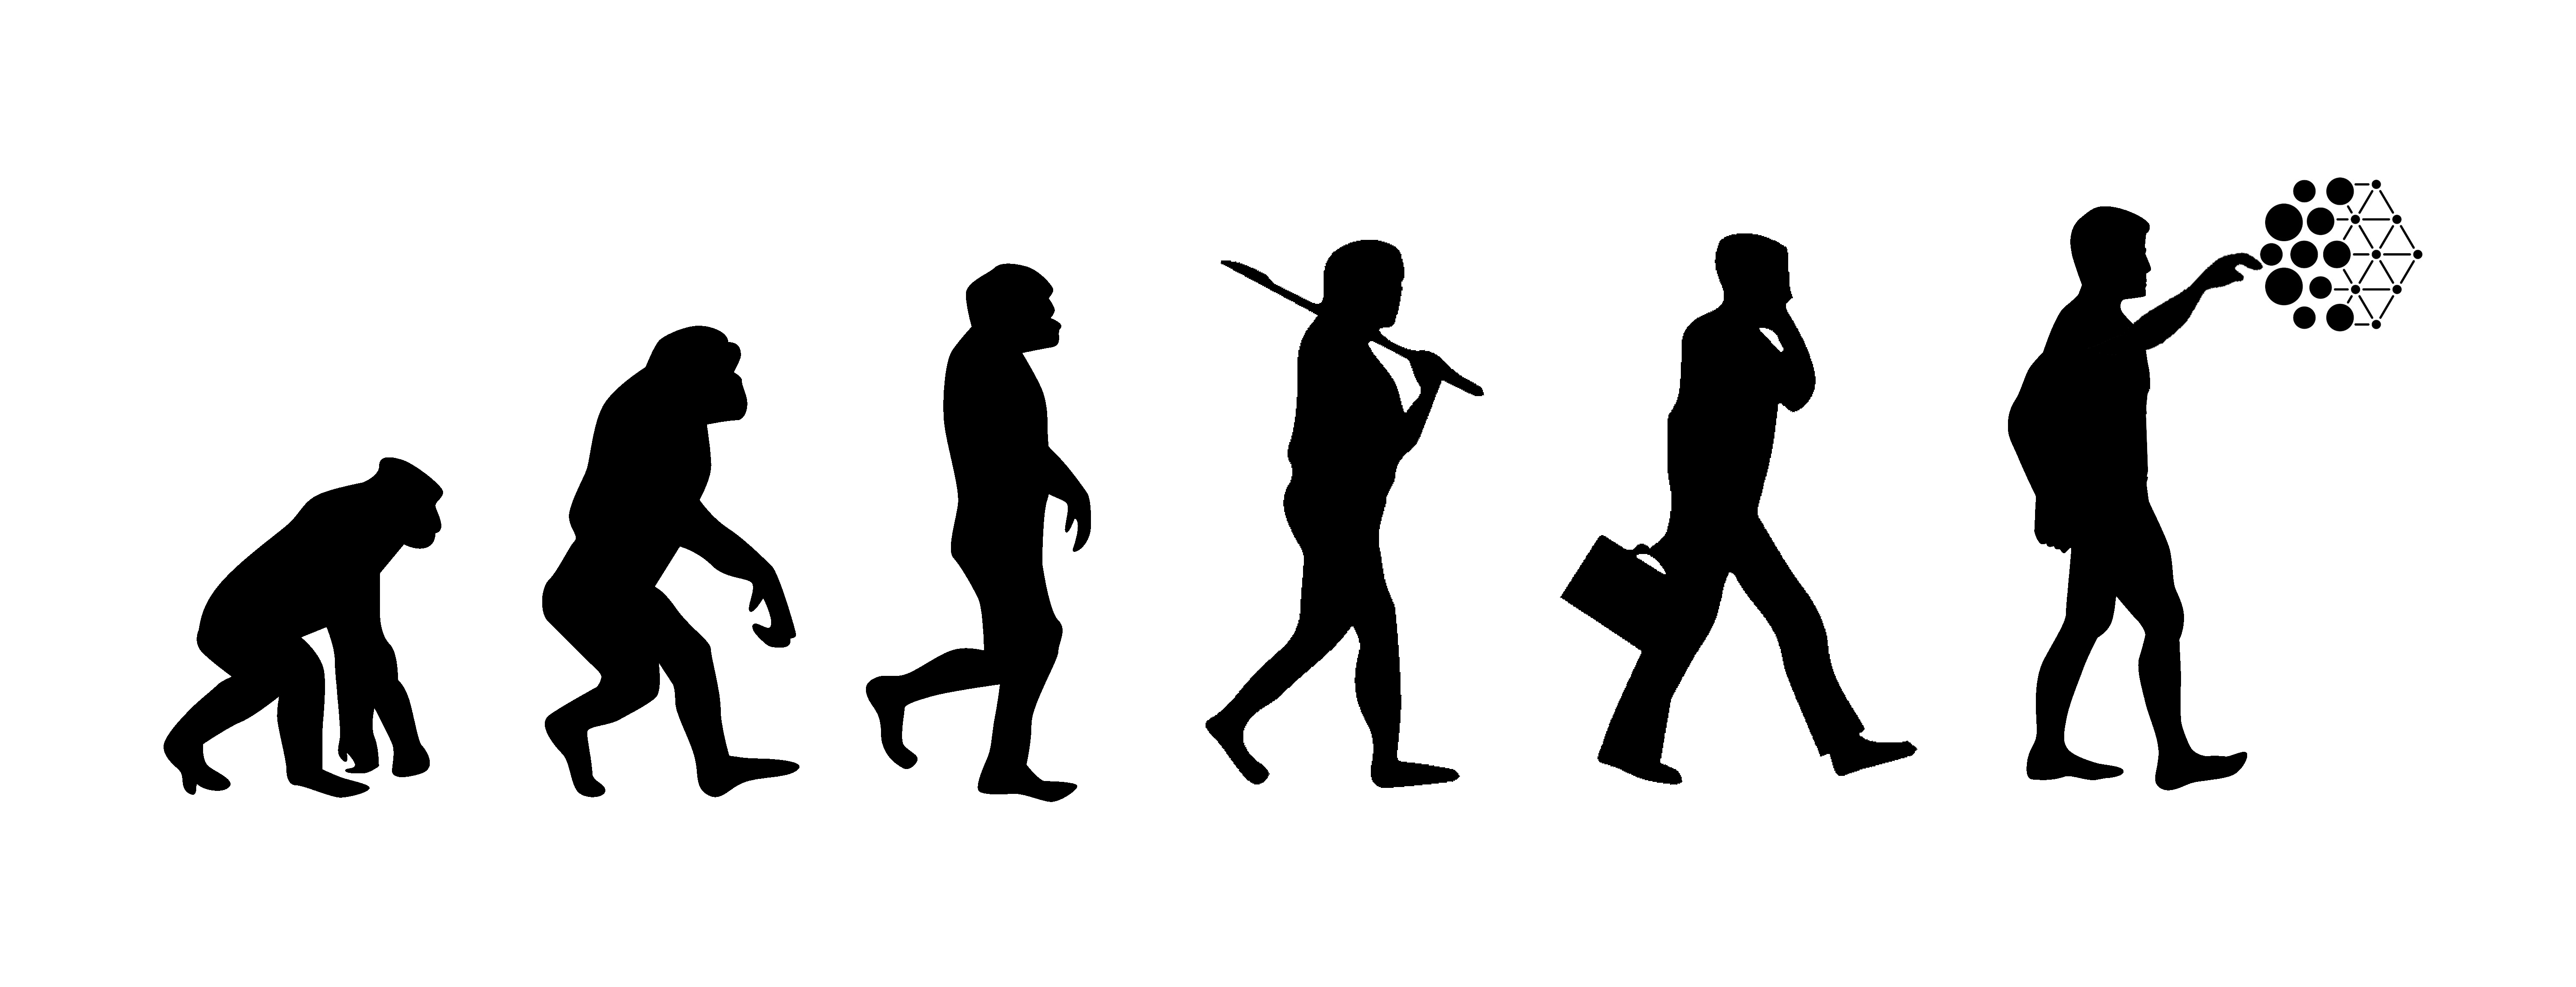
\includegraphics[width=0.90\textwidth]{../figures/evolution.png}
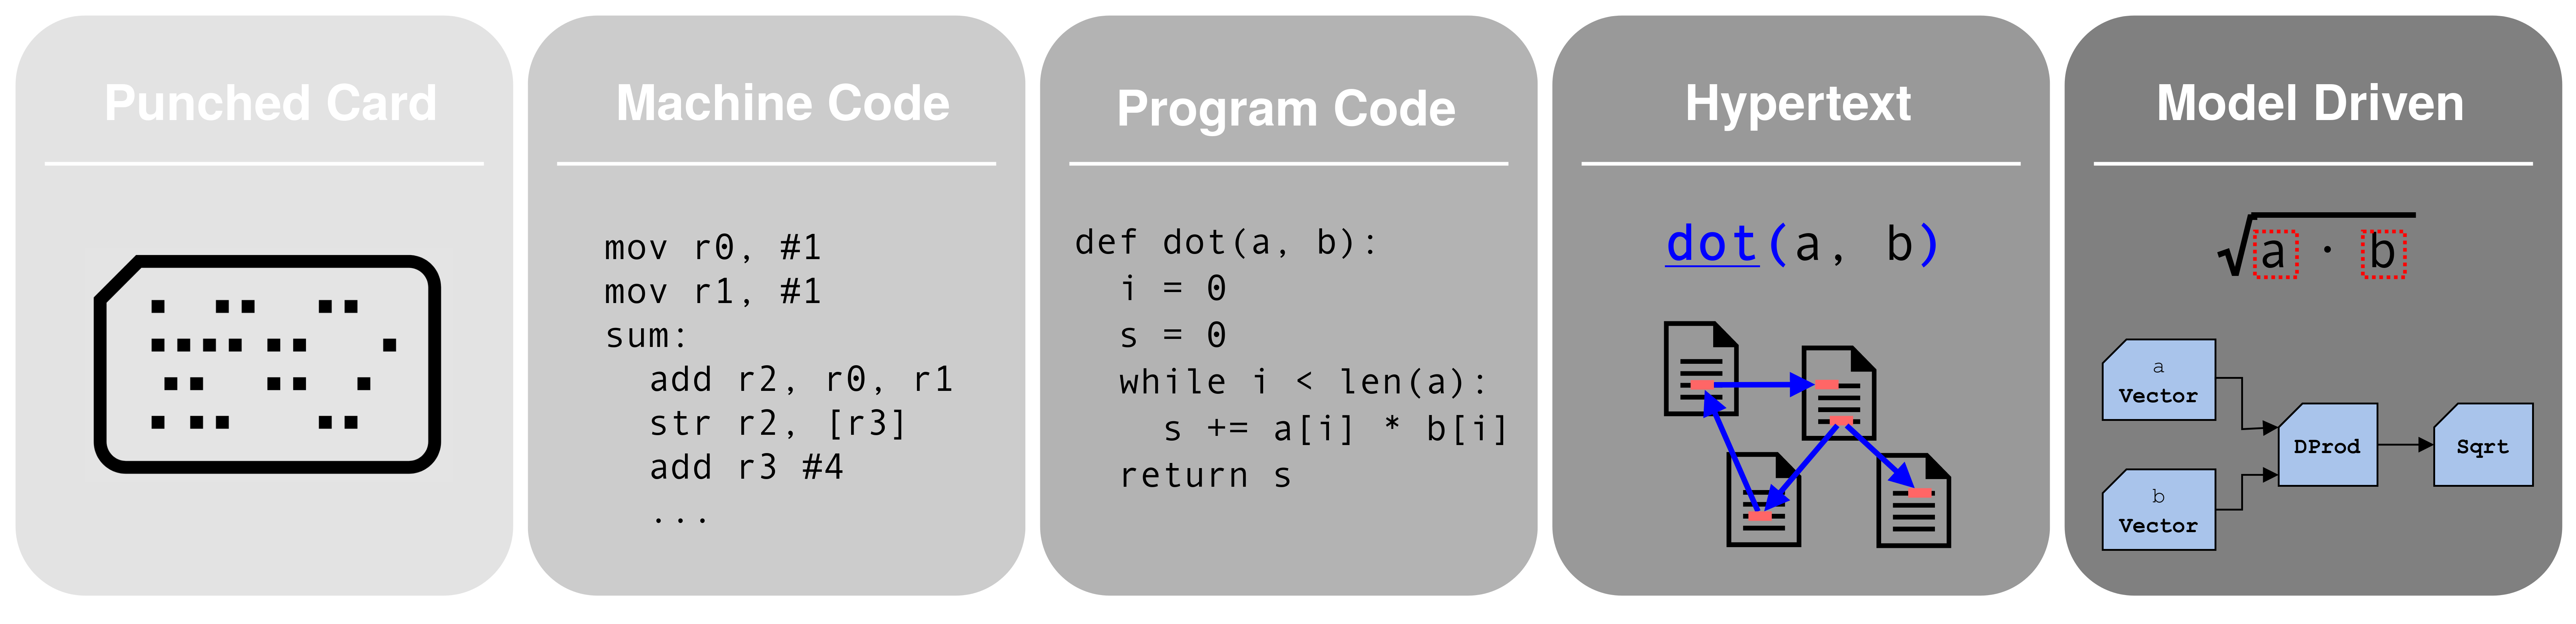
\includegraphics[width=0.90\textwidth]{../figures/progress_in_program.png}
\caption{The evolution of code. A gauche, les langues qui obligent l'utilisateur à s'adapter à la machine. À droite, on trouve des représentations de plus en plus souples du code source.}
\label{fig:evolution_of_programming}
\end{figure}

L'ASCII reste le support dominant de la programmation moderne, bien que les machines utilisent encore diverses formes de code assembleur de bas niveau pour l'exécution. Une grande partie de l'infrastructure logicielle est consacrée à la traduction entre ces représentations via les langages de programmation et les compilateurs. Bien que de nombreux cadres logiciels fournissent une interface de ligne de commande (CLI) minimale et que certains fournissent même des environnements de programmation sophistiqués, ces outils sont assez restrictifs. De la même manière que les premiers informaticiens n'ont probablement pas inventé de nouveaux algorithmes en imaginant des modèles de trous dans le papier, l'ASCII est également un moyen indirect d'exprimer des idées, bien qu'il soit un peu moins artificiel. Au fur et à mesure des progrès de la technologie matérielle et logicielle, les langages de programmation se sont déplacés "vers le haut de la pile", permettant à leurs utilisateurs d'exprimer des idées dans une notation plus familière et plus facile à raisonner sur son exécution.

\begin{figure}
\centering
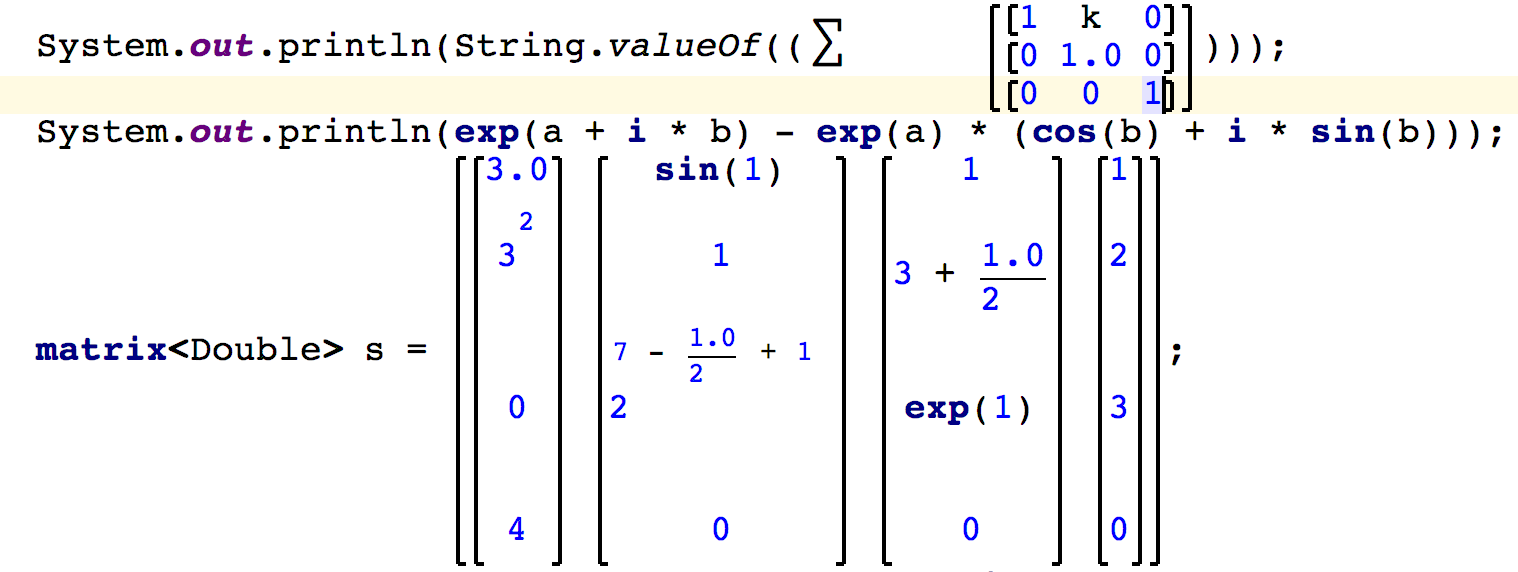
\includegraphics[width=0.90\textwidth]{../figures/mps_screenshot.png}
\caption{Projectional editors such as \href{https://www.jetbrains.com/mps/}{MPS}~\citep{voelter2010language, pech2013jetbrains} (ci-dessus) sont capables de rendre le code source de manière visuellement créative. Cela peut ressembler à la notation à main levée ou à un autre format visuellement attrayant.}
\label{fig:mps_screenshot}
\end{figure}

Avec le développement des langages modernes sont apparus des outils de programmation capables de représenter le code comme un mélange d'interfaces utilisateur hypertexte et graphique. Ces outils fournissent une représentation plus riche du code que le texte en clair et aident à saisir la structure graphique des programmes, mais utilisent toujours l'ASCII avec des indices visuels épars pour rendre le code. Certains outils prennent en charge de plus grands jeux de caractères et des ligatures typographiques basées sur des polices, bien que la représentation visuelle du code source reste essentiellement linéaire et textuelle.

Des interfaces utilisateur plus expérimentales, telles que proposées dans la littérature sur la programmation orientée langage~\citep{dmitriev2004language} et l'ingénierie guidée par modèle~\citep{famelis2015mummint}, suggèrent la possibilité de disposer de mises en page plus flexibles visuellement. Ce découplage entre la composition et la représentation du code source soulève de nombreuses questions intrigantes. Avec la prolifération des nouvelles abstractions et des abréviations de programmation, quel est le niveau de notation approprié requis pour une tâche de programmation donnée? Et quel est le public visé? Ce sont là des questions importantes à prendre en compte lors de la conception d'un nouvel outil de programmation.

Le plugin Hatchery fournit une interface graphique légère qui se superpose au code source du programme. Cette interface (\autoref{fig:hatchery_gui}) se compose principalement de simples repères visuels tels que la mise en évidence de texte, l'aide à la navigation et d'autres menus et panneaux de configuration permettant d'effectuer diverses tâches de programmation. L'EDI hôte offre un langage de conception composé d'iconographie et de motifs visuels répétitifs, qui servent de repères cognitifs pour guider la mémoire procédurale du développeur. La plateforme IntelliJ offre une palette d'éléments de conception communs, que les utilisateurs familiers avec l'EDI peuvent reconnaître d'un seul coup d'œil. Les plugins peuvent utiliser ces mêmes motifs pour accéder aux mémoires procédurales implantées dans la base d'utilisateurs, facilitant ainsi l'apprentissage par transfert. Hatchery fournit également un menu de paramètres pour la configuration et la gestion des installations ROS, qui peut détecter automatiquement les distributions ROS locales et permet également aux utilisateurs de configurer manuellement l'environnement \href{https://wiki.ros.org/ROS/Tutorials/InstallingandConfiguringROSEnvironment}{ROS}, comme indiqué dans et \autoref{fig:ros_settings}.
%
\begin{figure}[b]
\centering
\frame{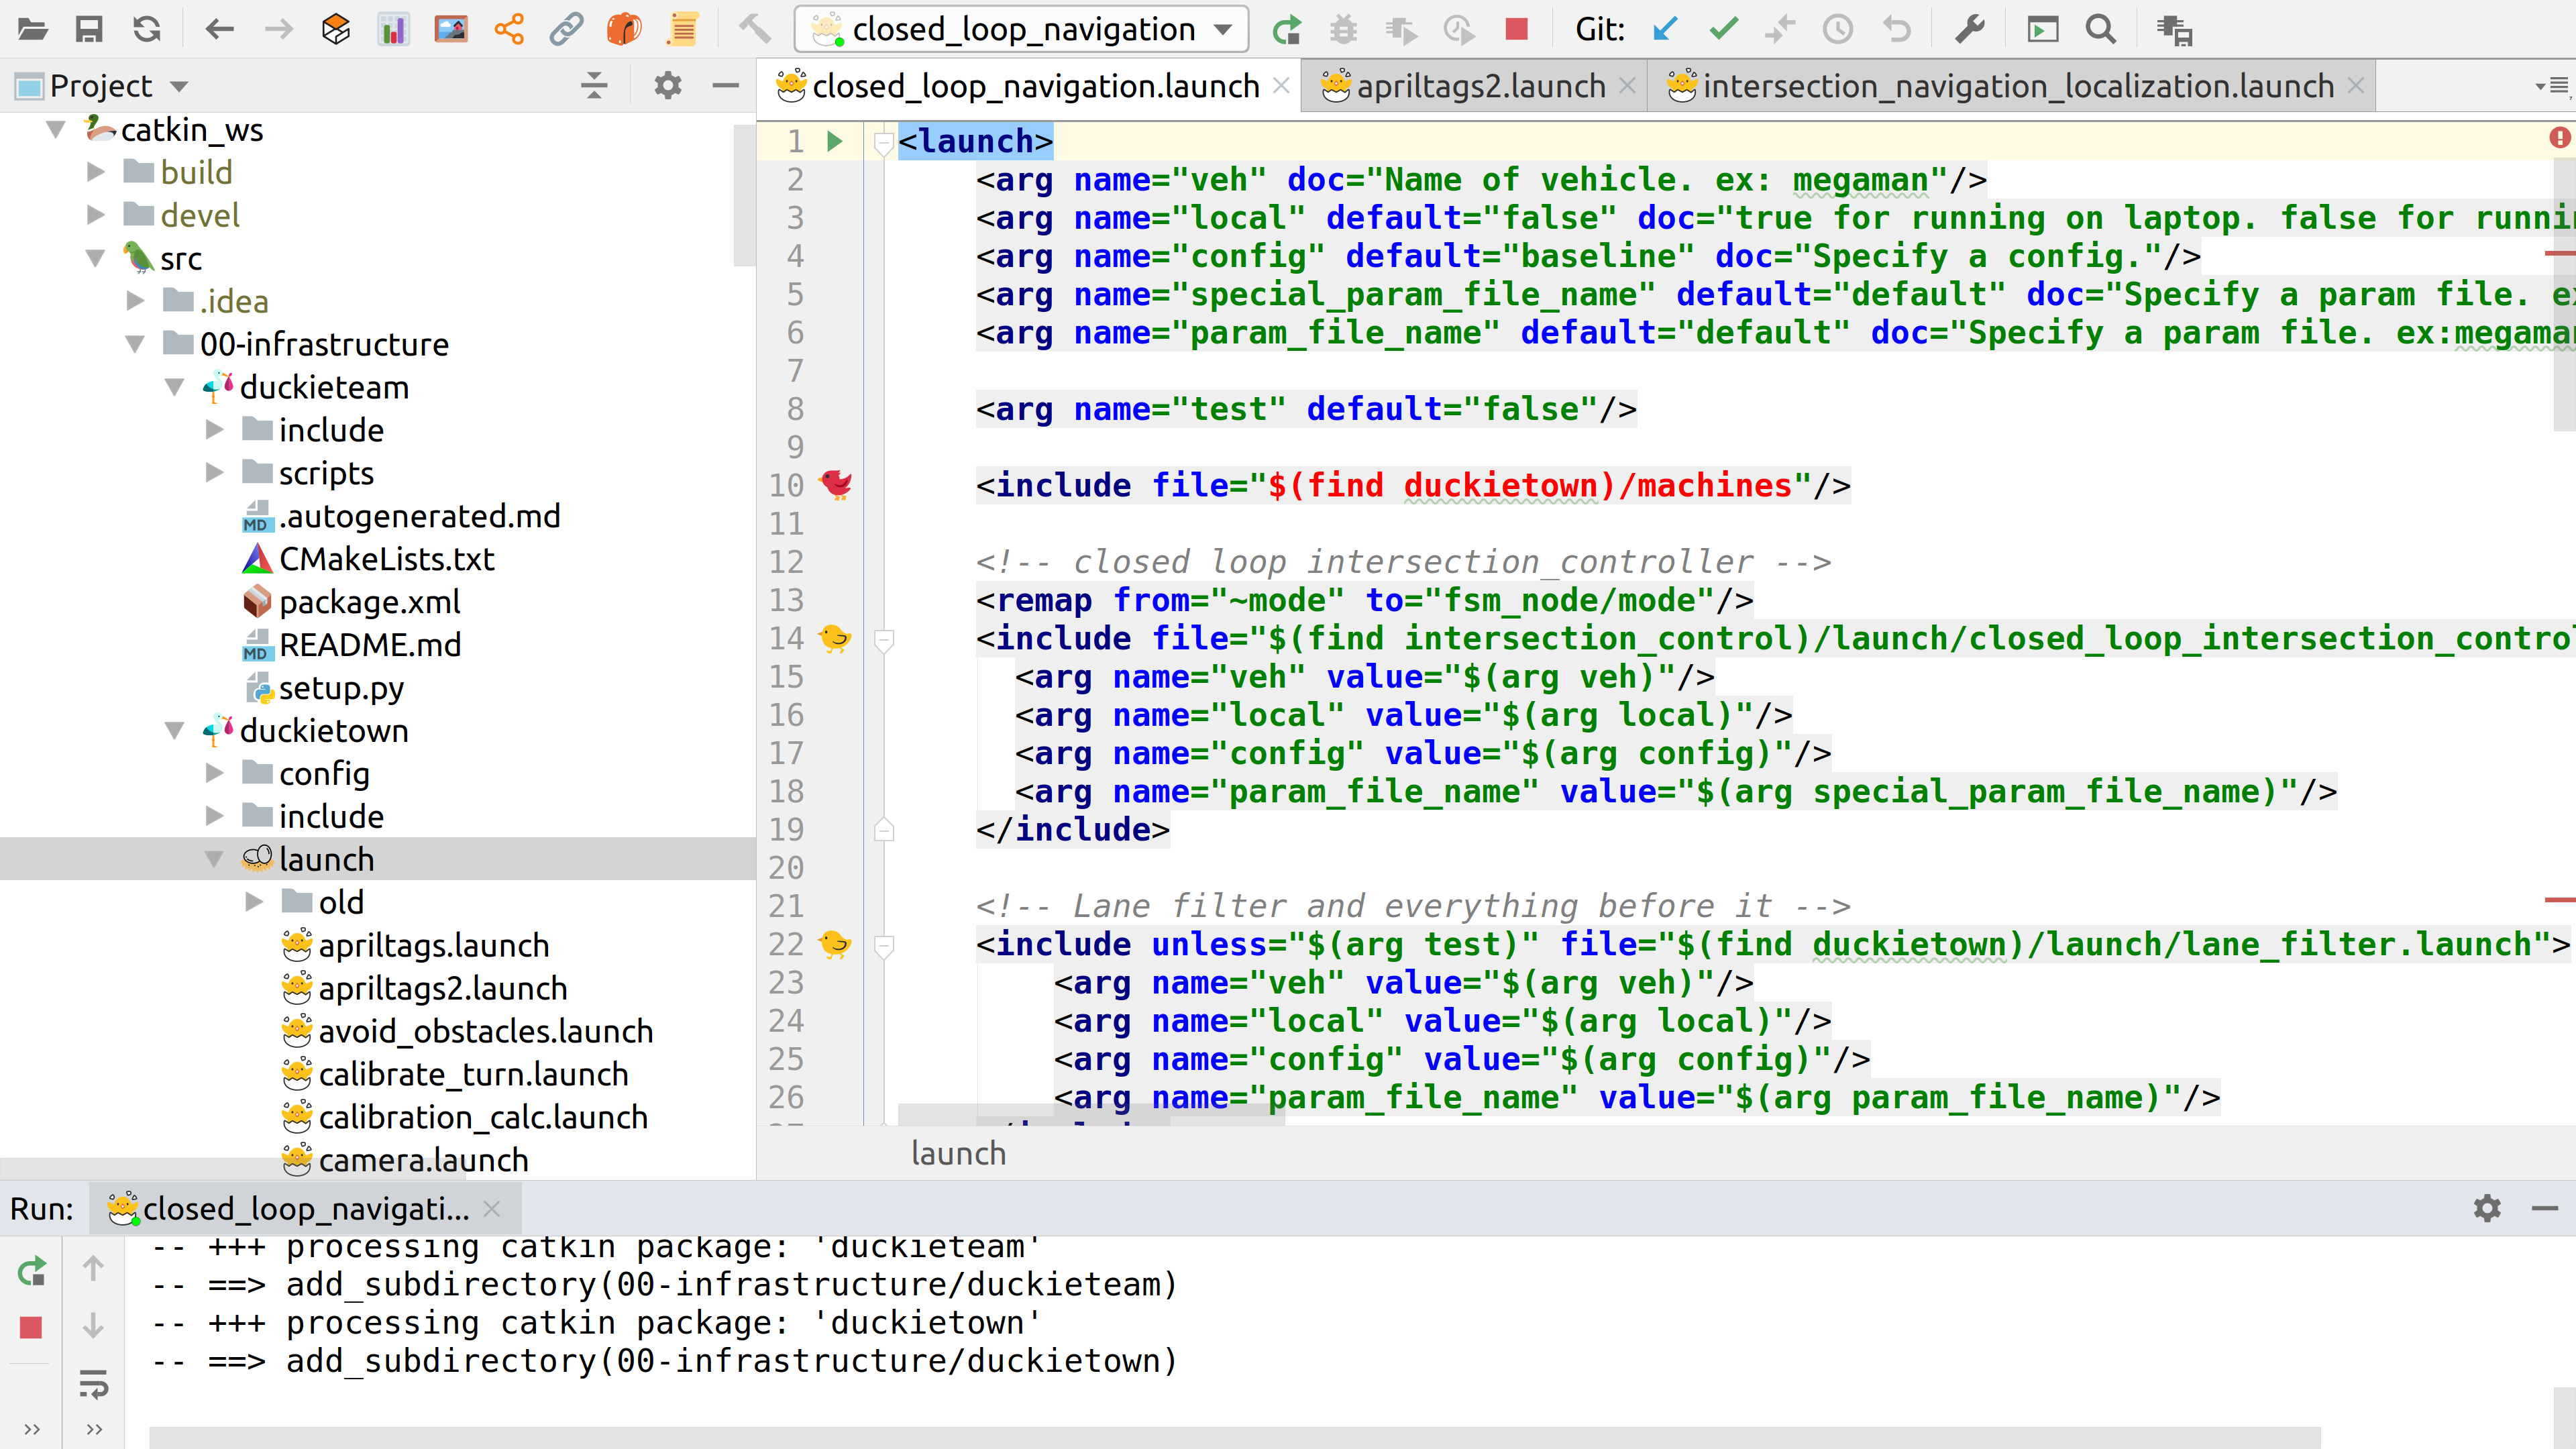
\includegraphics[width=0.90\textwidth]{../figures/hatchery_screenshot.png}}
\caption{Hatchery UI supports syntax highlighting, validation and project navigation.}
\label{fig:hatchery_gui}
\end{figure}
%
\begin{figure}
\centering
\frame{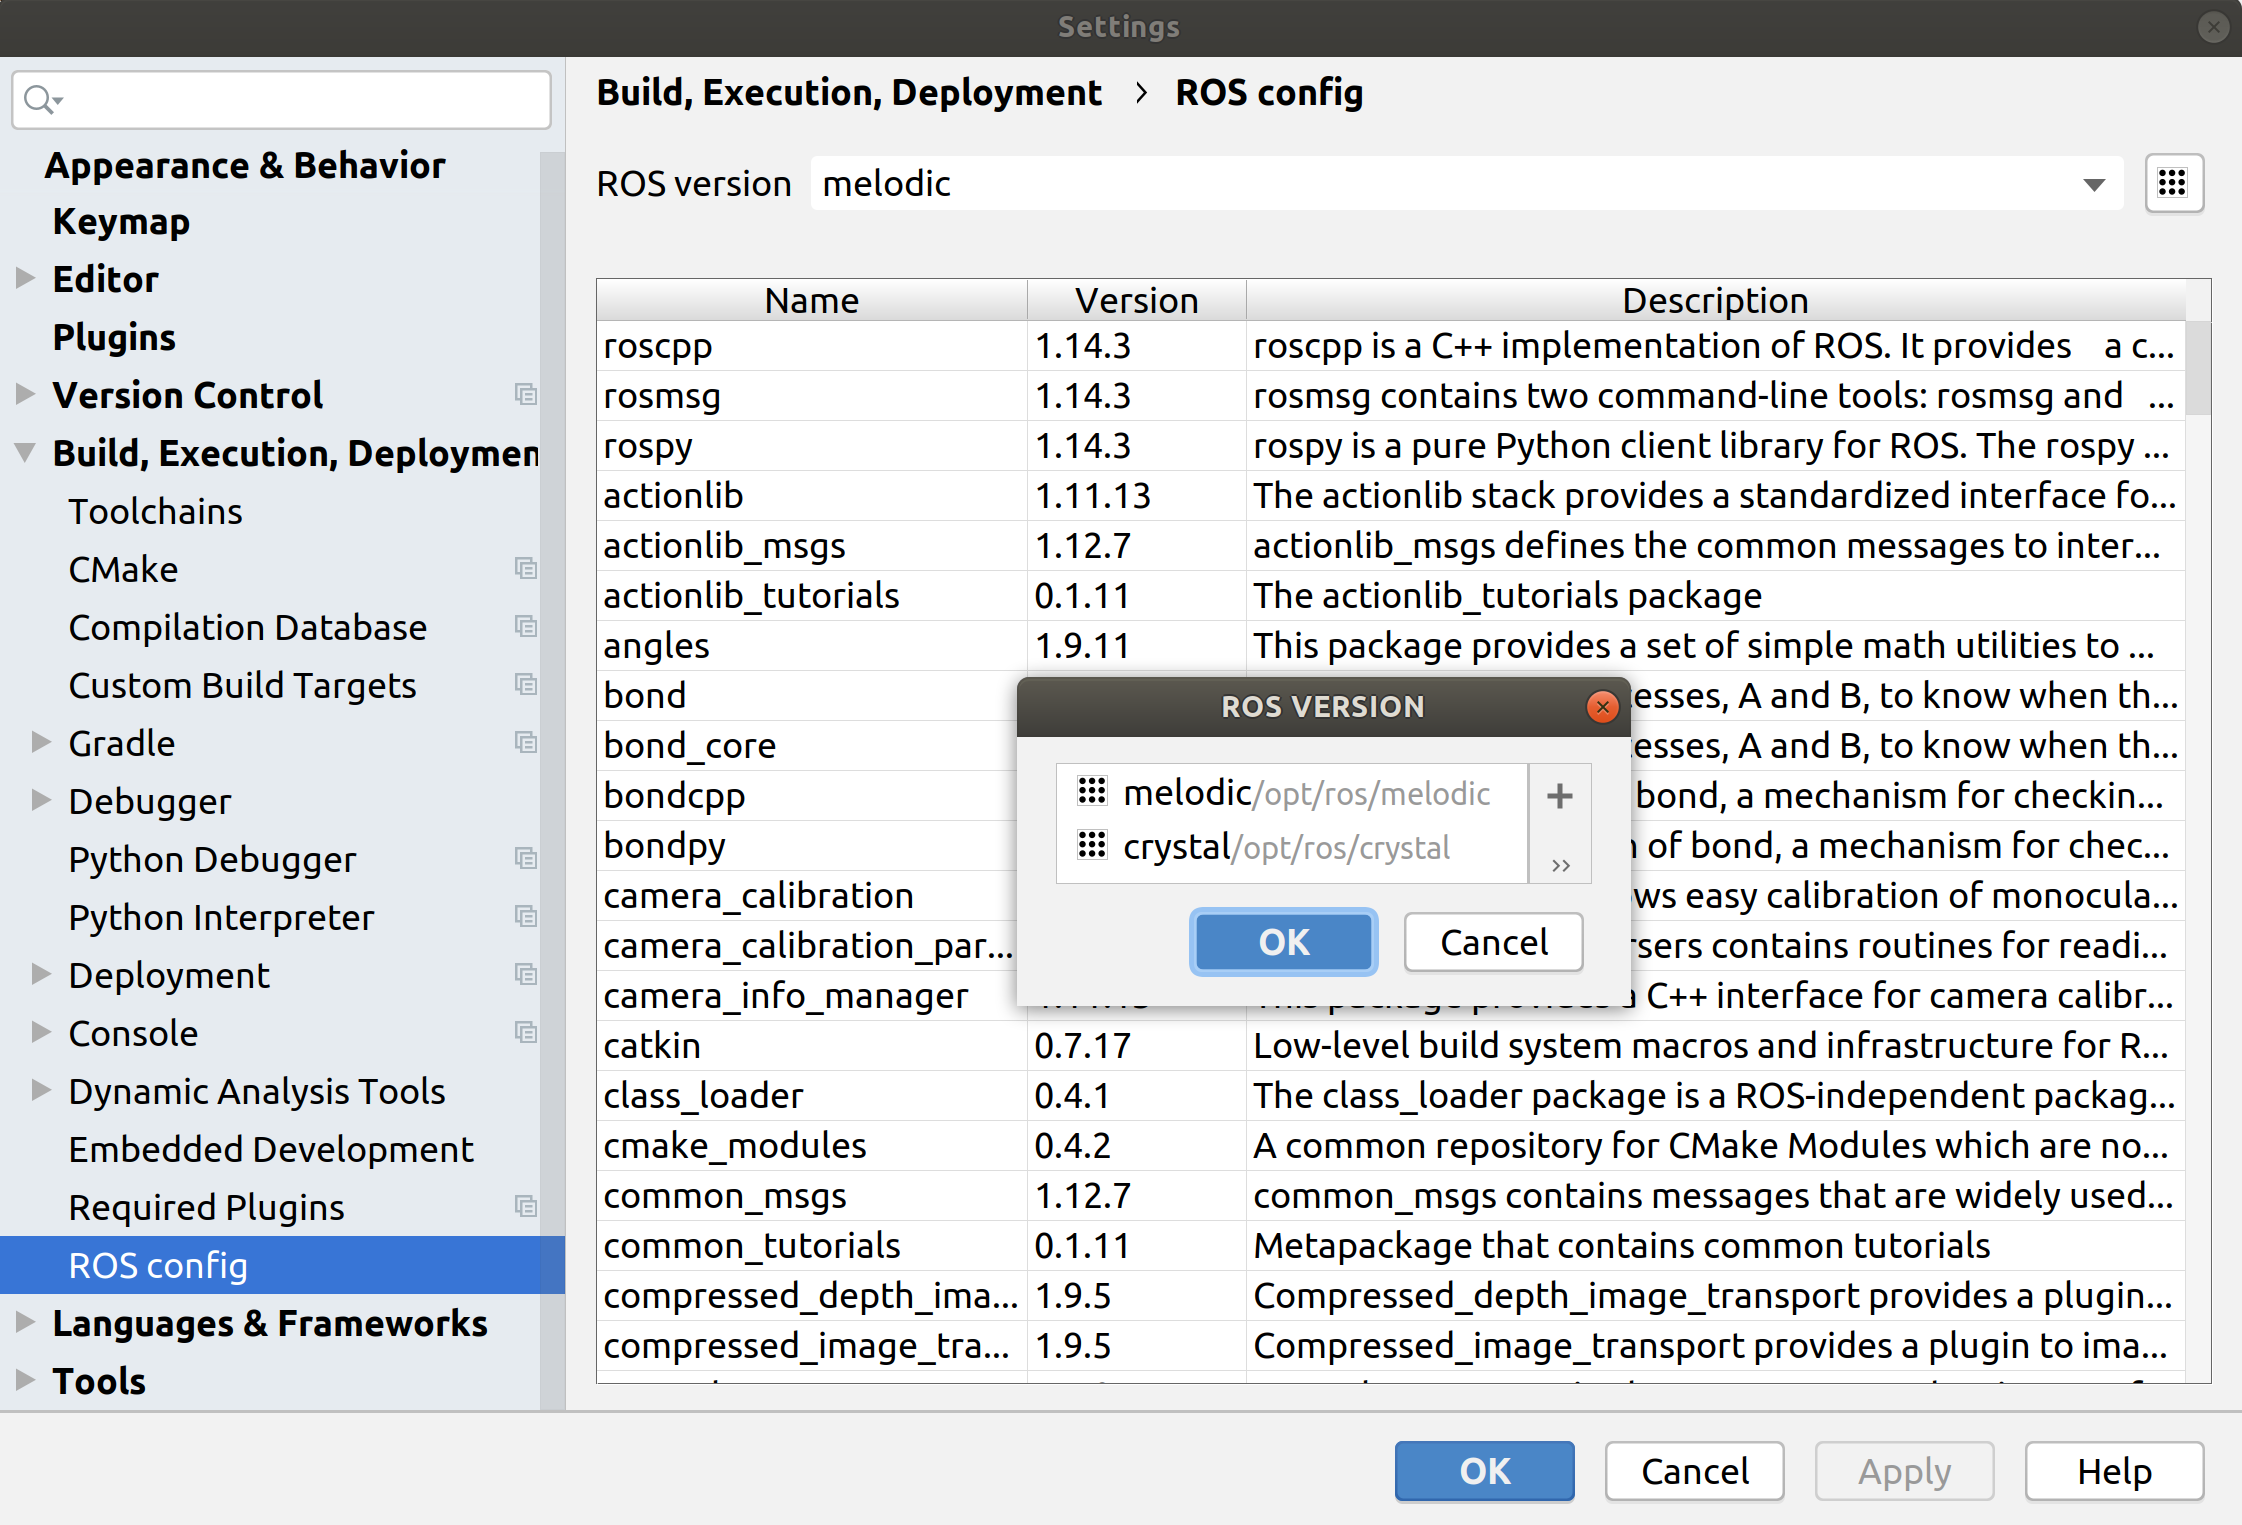
\includegraphics[width=0.90\textwidth]{../figures/ros_settings.png}}
\caption{Détection des packages ROS locaux. Accessible via: \menu{Fichier > Paramètres > ROS config}}
\label{fig:ros_settings}
\end{figure}

\section{Ouvres en cours}

\noindent Alors qu'il prend en charge de nombreux cas d'utilisation courante tels que la navigation en code rudimentaire, l'analyse statique et l'assistance à l'exécution, Hatchery est actuellement un travail en cours. Nous travaillons à étendre le support de Hatchery pour la programmation ROS dans certains des domaines suivants:\vspace{10pt}
%
\begin{itemize}
\item \textbf{Syntax support} -- Surlignage, navigation, autocomplétion
\item \textbf{Analyse des programmes} -- Inspections du code, intentions et peluches
%\item \textbf{Testing support} -- Tests d'unité et d'intégration, couverture de code
\item \textbf{Création de projet} -- Configuration du projet et génération de code passe-partout
\item \textbf{Gestion des dépendances} -- Suivi des paquets installés et manquants
\item \textbf{Surveillance des outils} -- Enregistrement, diagnostic, profilage et visualisation
\item \textbf{Crash analytics} -- Tracés de pile améliorés avec navigation des sources
\item \textbf{Build automation} -- Delta rebuilds, cmake magic, code hotswap
%\item \textbf{intégration ROS} -- Nœuds, sujets, services, paramètres, graphiques
%\item \textbf{Duckumentation} -- Instructions d'utilisation et fonctionnalités supportées
\end{itemize}\vspace{10pt}
%
Une liste plus complète des fonctionnalités actuellement prises en charge et à venir est détaillée ci-dessous:\vspace{10pt}
%
\begin{multicols}{2}
\begin{todolist}
\item[\done] ROS Launch (\href{https://wiki.ros.org/roslaunch/XML}{\inline{*.launch}}, \href{https://wiki.ros.org/rostest/Writing}{\inline{*.test}})
\begin{todolist}
\item[\done] La coloration syntaxique
\item[\done] Références de ressources (\inline{\$(find <directory>)...})
\end{todolist}
\item[\done] \href{https://wiki.ros.org/Manifest}{Manifeste de paquet (\inline{package.xml})}
\begin{todolist}
\item[\done] Coloration syntaxique
\item[\done] \href{https://wiki.ros.org/catkin/package.xml#Dependencies}{Dépendances des paquets} (\inline{<build\_depend>}, \inline{<test\_depend>}, \inline{<run\_depend>})
\end{todolist}
\item[\done] ROS URDF (\inline{*.urdf.xacro})
\begin{todolist}
\item[\done] Coloration syntaxique
\item[\done] Références de ressources (\inline{\$(find <directory>)...})
\end{todolist}
\item[\done] \href{https://wiki.ros.org/Bags/Format}{ROS Bag (\inline{*.bag})}
\begin{todolist}
\Mise en évidence syntaxique
\end{todolist}
\item[\done] \href{https://wiki.ros.org/msg}{Message ROS (\inline{*.msg})}
\item[\done] \href{https://wiki.ros.org/srv}{Service ROS (\inline{*.srv})}
\item[\done] Mettre en œuvre la structure de l'avant-projet et le support XML
\item[\done] Écrire une application MVP/POC qui prend en charge le renommage et le remaniement des fichiers
\item[\done] Ajouter le support pour les modèles de projets et la création de projets squelettes
\item[\done] Ajouter un support pour le déploiement d'un projet depuis la machine locale vers la machine distante
\item[\done]Ajouter un support pour la surveillance et le suivi du code en cours d'exécution, la visualisation des journaux
\begin{todolist}
\item Suivi du fichier de suivi en direct
\item Enregistrer sur le disque local
\item Recherche dans le journal
\end{todolist}
\item Collecter les crash dumps et les relier aux points de code correspondants
\begin{todolist}
\item Lier les traces de la pile au code source
\item Copier les infos sur l'environnement et crash dump dans le presse-papiers
\end{todolist}
\item Intégration avec le \href{https://www.ros.org}{Système d'exploitation du robot} (ROS)
\begin{todolist}
\item[\done] ROS 1 support (\href{https://wiki.ros.org/kinetic}{Kinetic Kame} recommandé)
\item \href{https://github.com/ros2/ros2/wiki}{ROS 2} support
\item[\done] Gestion des installations ROS.
\end{todolist}
\item[\done] \href{http://gazebosim.org/}{Gazebo} intégration du simulateur
\item CMake build integration
\item Support de débogage à distance
\item Intégration des dockers
\begin{todolist}
\item[\done] Soutien de base aux dockers
\item Support à distance de l'hôte et du script
\item \href{https://hub.docker.com}{Docker Hub} sensibilisation à l'espace de noms
\item Support pour l'outillage \href{https://platformio.org}{platformio}
\item X11 forwarding and \href{https://wiki.ros.org/rqt}{rqt} support
\end{todolist}
\item Analyse statique pour une utilisation abusive de \href{https://wiki.ros.org/rospy}{Python API}
\begin{todolist}
\item Détection de dépendance invalide
\item Validate \inline{.msg}/\inline{.srv} compatibility
\item ROS nodes and graph analysis via \href{https://wiki.ros.org/rosdep}{\inline{rosdep}}/\href{https://wiki.ros.org/rqt_dep}{\inline{rqt\_dep}}
\end{todolist}
\item[\done] \href{https://wiki.ros.org/rqt}{rqt} support de plugin
\begin{todolist}
\item[\done] \href{https://wiki.ros.org/rqt_image_view}{\inline{rqt\_img\_view}} - Voir les images
%\item[\done] \href{https://wiki.ros.org/rqt_plot}{\inline{rqt\_plot}} - Tracez les données visuellement
\item[\done] \href{https://wiki.ros.org/rqt_graph}{\inline{rqt\_graph}} - Messages graphiques
\item[\done] \href{https://wiki.ros.org/rqt_dep}{\inline{rqt\_dep}} - Visualiser les dépendances
%\item[\done] \href{https://wiki.ros.org/rqt_bag}{\inline{rqt\_bag}} - Reproduire et modifier les fichiers de poche
%\item \href{https://wiki.ros.org/rqt_common_plugins}{rqt\_common} - Plugins communs
\end{todolist}
\end{todolist}
\end{multicols}

\section{Futurs travaux}

Les plugins EDI comme Hatchery améliorent la productivité des développeurs et la qualité des logiciels dans les langages et cadres de travail spécifiques à un domaine. La clé de ce processus est le développement d'analyseurs personnalisés capables d'analyser le code et de détecter les erreurs courantes, ce qui nécessite une connaissance du modèle de programmation ROS. Alors que les cadres spécifiques à un domaine comme les ROS sont devenus de plus en plus polyvalents, le développement et la maintenance des analyseurs qui les prennent en charge peuvent être difficiles, surtout lorsque ces cadres se développent et évoluent. Nous pensons que l'analyse syntaxique est essentiellement une compétence qui peut être apprise à partir d'exemples. Nous étudions actuellement les moyens d'automatiser le développement de générateurs d'analyseurs sensibles au contexte pour des applications agnostiques au domaine. Nous pensons que cette approche peut être adaptée à un cadre de méta-apprentissage qui est capable d'être transféré d'un domaine à l'autre et nécessite beaucoup moins de connaissances humaines.

\section{Conclusion}

Dans ce chapitre, nous démontrons l'intérêt des EDI pour le développement de logiciels à usage général et nous présentons un plugin EDI spécifique à un domaine pour le développement de la robotique, développé à l'origine comme projet final dans la classe Duckietown~\citep{paull2017duckietown}. En utilisant Hatchery, les développeurs peuvent recevoir de l'aide pour écrire, compiler et exécuter des applications ROS, un cadre middleware populaire pour le développement de la robotique, en utilisant la plateforme IntelliJ. Il offre un support pour l'analyse syntaxique et l'analyse statique des fichiers de configuration ROS, ainsi qu'une assistance pour l'exécution et le débogage des applications ROS. L'auteur souhaite exprimer sa gratitude à \href{https://github.com/paoloach}{Paolo Achdjian} pour sa contribution à plusieurs fonctionnalités, notamment un menu de configuration et de paramètres d'exécution personnalisés. Pour plus d'informations sur Hatchery, veuillez consulter le site \url{https://github.com/duckietown/hatchery}.